\chapter{\iflanguage{ngerman}{Netzwerkkommunikation und Datenaustausch}{Network communication}}
\label{sec:overview}

Ein digitaler Datenbus der alle Daten in Echtzeit zu Verfügung stellt und die Steuerung der medizinischen Geräte im OP-Saal über einen zentralen Zugriffspunkt, ist noch nicht die Realität. Netzwerkkommunikation und Datenaustausch zwischen den medizinischen Geräten im OP-Saal werden durch herstellerabhängige Schnittstellen eingeschränkt. Bei der Installation eines Hybriden OP-Saals, muss im Voraus ein Hersteller gewählt werden, denn \glqq eine Integration von Drittanbieterkomponenten kann nur in Kooperation mit dem Hersteller des Integrationssystems erfolgen\grqq{} \cite{DerDigitaleOperationssaal}.

Um diesem Problem entgegen zu wirken, wurde für eine herstellerübergreifende Netzwerkkommunikation die Service Oriented Architecture für den medizinischen Gebrauch angepasst. Des Weiteren sollen Standards wie DICOM, HL7 und IHE zum ungehinderten Datenaustausch beitragen.

\subsection{Service Oriented Architecture}

\begin{figure} [H]
	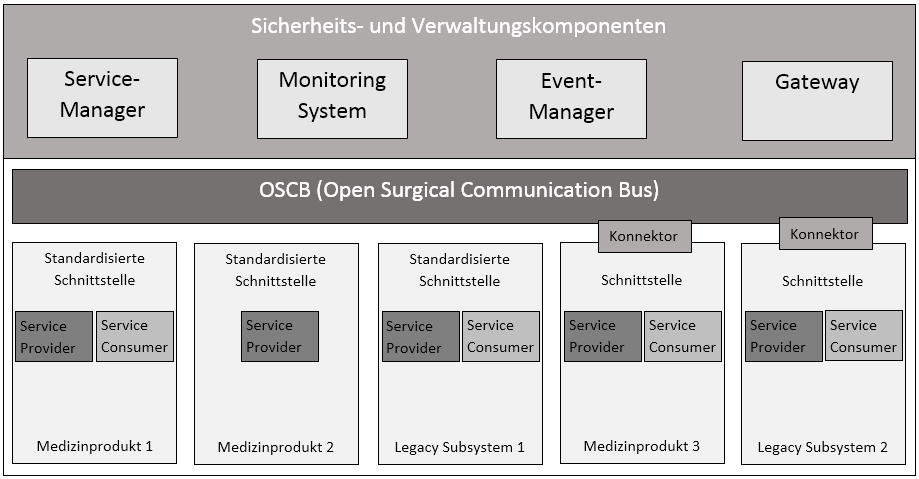
\includegraphics[scale = 0.6]{Content/Pictures/soa-red.png}
	\caption{SOA für den medizinischen Gebrauch im Operationssaal nach Abbild \cite{DerDigitaleOperationssaal}.}
	\label{fig:soa}
\end{figure}

In der Service Oriented Architecture (SOA, Abb. \ref{fig:soa}) für den medizinischen Gebrauch, interagieren Service Provider und Service Consumer über einen Open Surgical Communication Bus (OSCB). Dabei können medizinische Geräte sowohl Service Provider als auch Consumer sein und Dienste über eine standardisierte Schnittstelle nutzen bzw. bereitstellen. Der Service Manager verwaltet alle verfügbaren Geräte und Dienste im Netzwerk. Service Consumer können über den Service Manager Dienste anfragen, welcher verfügbare und passende Service Provider zur Verfügung stellt. Die Kommunikation läuft daraufhin direkt zwischen Consumer und Provider ab \cite{DerDigitaleOperationssaal}. \\ 
Für den Informationsaustausch sind standardisierte herstellerübergreifende Schnittstellen essentiell. Für Geräte die keine standardisierte Schnittstelle (wie DICOM) zu Verfügung stellen, übernimmt ein Konnektor die Aufgabe der Transformation. Damit wird eine höhere Bandbreite an Geräten unterstützt, welche in die SOA integriert werden können. Jegliche Kommunikation über den OP-Saal hinaus mit anderen Klinik-IT Netzwerken, wird über eine Gateway geleitet. So können die vorschriftsgemäßen Sicherheitsansprüche gewährleistet werden. Weitere optionale Komponenten sind der Event Manager und das Monitoring System. Der Event Manager verwaltet auftretende Ereignisse und informiert gegebenenfalls andere Geräte über diese. Das Monitoring System ist zur Unterstützung des Service Managers, für die Überwachung der angeschlossenen Geräte und um gegebenenfalls fehlerhafte Services zu identifizieren \cite{DerDigitaleOperationssaal}. 

Webservices bieten sich durch ihre lose Client-Server-Kopplung und Erweiterbarkeit für die Umsetzung der SOA im medizinischen Bereich an. Zur Verwirklichung des OSCBs ist Ethernet, aufgrund der hohen Bandbreite und der bereits bestehenden Infrastruktur in Krankenhäusern, die Grundlage für die Vernetzung. Die Gewährung der Sicherheit und Zuverlässigkeit des Systems ist mit einem höheren Aufwand verbunden als bei anderen Technologien. Die tatsächliche Client-Server-Kommunikation wird dann je nach Anwendungsfall mit TCP oder UPD verwirklicht \cite{DerDigitaleOperationssaal}.

Dieser Ansatz der Umsetzung einer SOA im medizinischen Umfeld, ermöglicht alle Geräte im Netzwerk über einen zentralen Zugriffspunkt im Operationssaal zu kontrollieren. Dazu gehören die bildgebenden Verfahren, aber auch der OP-Tisch, die Beleuchtungsanlagen und die Kameras mit der Anzeigeausgabe auf den Monitoren \cite{DerDigitaleOperationssaal}.

OR.NET (Secure Dynamic Networking in Surgery and Clinic) ist ein Projekt welches auf der SOA basiert und die Integration von medizinischen Geräten und IT-Systemen demonstriert. Ziel ist es, die Gerätekommunikation im OP zu erleichtern indem  Echtzeitkommunikation ermöglicht und eine internationale Normung für alle OP-Säle festgelegt wird. Zur Umsetzung dieses Projekts wurde ein Substandard entwickelt. Dieser soll nicht bereits vorhandene Standards wie HL7 oder DICOM ersetzen, sondern Geräte und Systeme in das IT-Netzwerk einbinden, welche die genannten Standards nicht umsetzen können \cite{ORnetWebsite}.\\
Zur Demonstration der Funktionsweise und Umsetzbarkeit von OR.NET wurden OP-Säle errichtet (Abb. \ref{fig:ornet}), die medizinische Geräte und klinische IT-Systeme von unterschiedlichen Herstellern vereinen \cite{ORnet}. Damit konnte gezeigt werden, dass eine einheitliche Mensch-Maschine-Interaktion unabhängig vom Hersteller möglich ist. Durch die Vernetzung kann während einer Operation auf präoperativ angefertigte Bilddateien, Patienteninformationen und Laborbefunde zugegriffen werden. Auch von außerhalb des OP-Saals können die Informationen eingesehen werden, die im OP-Saal erfasst und aufgezeichnet wurden \cite{ORnetWebsite}.

\begin{figure} [t!]
	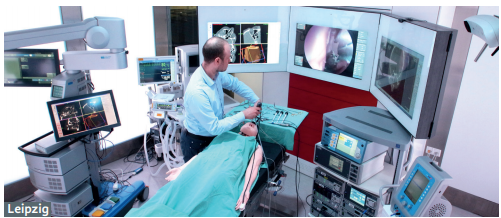
\includegraphics[scale = 0.8]{Content/Pictures/ornet.png}
	\caption{Operationssaal zur Demonstration von OR.NET in Leipzig, der für die Kopf- und Halschirurgie ausgelegt wurde \cite{ORnetWebsite}.}
	\label{fig:ornet}
\end{figure}

\subsection{Medizinische Standards}

Zur Kompatibilität medizinischer Geräte und Systeme unterschiedlicher Hersteller wurden Standards definiert, die erläutert werden sollen.

Einer der am Weitesten verbreiteten Standards ist DICOM (Digital Imaging and COmmunications in Medicine). DICOM ist ein schnittstellenkompatibles Datenformat für die digitale medizinische Bildgebung. Es fungiert dabei als Bildformat, wird aber auch zum senden, verteilen und speichern medizinischer Bilderdateien verwendet die von den bildgebenden Geräten (wie CT, MRT, US,..) erzeugt werden. Dabei ist das Dateiergebnis unabhängig von Aufnahmegerät und Hersteller. DICOM ist darüber hinaus für die Darstellung der Bilder verantwortlich und ermöglicht nachträgliche Bildverarbeitung. Zusätzlich bietet dieser Standard Vorteile für die Dokumentation und Anzeige von medizinischen Bilddateien. So werden bei DICOM Dateien bis zu 65.536 (16 Bit) unterschiedliche Grauschattierungen unterstützt, wobei im Gegensatz dazu bei JPG nur 256 (8 Bit) möglich sind \cite{DICOM}. Das verhilft Details im aufgenommenen Bild korrekt darzustellen und für den Chirurgen erkenntlich zu machen. Zu jeder aufgenommenen Bilddatei werden Daten, wie die Patienteninformationen oder Position des bildgebenden Geräts während der Aufnahme, gespeichert \cite{DICOM}.

Ein weiterer Standard ist HL7 (Health Level Seven). HL7 ist ein schnittstellenkompatibler Kommunikationsstandard wie DICOM \cite{DerDigitaleOperationssaal}. Dieser bietet Protokolle für den Austausch, die Integration, Abfrage und Organisation von digitalen Gesundheitsinformationen, die keine Bilddateien sind. Es wird festgelegt, mit welcher Sprache, Struktur und welchen Datentypen Informationen in Pakete verpackt und versendet werden \cite{HL7}.

PACS (Picture Archiving Communication System) ist zur Darstellung, Analyse, Manipulation und zur Langzeitarchivierung der Bild- und Patientendaten. Nachdem die Daten von einem Gerät erfasst werden, stehen sie im Netzwerk zur Verfügung und können von mehreren Zugriffspunkten eingesehen werden \cite{PACS}.
Die Bilder im DICOM Format werden über das DICOM Netzwerk übertragen und von PACS als DICOM Objekte komprimiert und archiviert \cite{DICOM}.

Die genannten Standards weisen im Zusammenspiel Limitierungen auf. Aus diesem Grund wurde IHE (Integrating the Healthcare Enterprise) entwickelt. IHE baut auf Standards wie DICOM und HL7 auf und soll das Zusammenwirken sowie die Kommunikation unterschiedlicher IT-Systeme im medizinischen Umfeld verbessern \cite{DICOMundIHE}. 
IHE ist eine Initiative von Gesundheitsexperten einen weiteren Kommunikationsstandard zu entwickeln, um die Art und Weise zu verbessern, wie Computersysteme miteinander interagieren und Informationen austauschen. Mit diesem Standard wird die Kommunikation zwischen unterschiedlichen Systemen verbessert, ist einfacher zu implementieren und ermöglicht Informationen effektiver zu nutzen \cite{IHE}.

Die Kombination der genannten Standards kann die Kompatibilität herstellerübergreifender Geräte und Systeme realisieren. 
Die Ausstattung eines OP-Saals kann somit flexibel ausgewählt werden \cite{DerDigitaleOperationssaal}.

\subsection{Sicherheitsprobleme und Datenschutz}

Mit der Digitalisierung und Vernetzung der Geräte und Systeme im Operationssaal, ist die Gewährleistung der Sicherheit und des Datenschutzes ein wichtiges Thema geworden.
Durch die Einbindung der medizinischen Geräte in das Netzwerk, sind diese neuen Gefahren ausgesetzt und es müssen Schutzmaßnahmen ergriffen werden. Wie bereits in der SOA erläutert, findet jegliche Kommunikation über den Operationssaal hinaus über ein Gateway statt. Eine Firewall wird eingesetzt, um den Datenverkehr zwischen dem OP- und Klinik-Netzwerk zu überwachen und gegebenenfalls Angriffe von außerhalb abzuwehren. Zur Gewährleistung von Sicherheit und Datenschutz muss auch sichergestellt werden, dass \glqq ein Medizingerät nur authentisierte, verifizierte und validierte Befehle entgegennimmt und ausführt\grqq{} \cite{DerDigitaleOperationssaal}. \\
Besonders im Bezug auf Datenschutz ist eine \glqq vertrauliche Übermittlung von sensiblen Daten wie Patientenidentität, Vitalparameter, Krankengeschichte und Medikation unerlässlich\grqq{} \cite{DerDigitaleOperationssaal}. Deshalb müssen die Geräte und Daten vor unerlaubten Lese- und Schreibzugriffen geschützt werden. \\
Die übermittelten Dateiformate bieten von sich aus keine Schutzmechanismen. Das wird deutlich, wenn eine DICOM Datei in einem Editor wie Wordpad betrachtet wird. Private und sensible Daten, wie den Patientennamen, behandelnden Arzt und das Krankenhaus, sind öffentlich lesbar und änderbar (Abb. \ref{fig:dicom}). Darüber hinaus kann das DICOM Bild mit passender Software betrachtet, bearbeitet oder ausgetauscht werden \cite{DICOM}.\\

Aus diesem Grund müssen das Netzwerk und die versendeten Daten vor unberechtigtem Zugriff und Manipulation geschützt und gegebenenfalls anonymisiert werden. Konkret findet jegliche Kommunikation über ein VPN (Virtual Private Network) statt und alle Computer im Netzwerk sind mit einer Firewall ausgestattet. Zur Sicherstellung von Integrität und Vertraulichkeit werden alle Nachrichten signiert und verschlüsselt \cite{DerDigitaleOperationssaal}. Darüber hinaus wir vor jeden Lese- und Schreibzugriff, das Zugriffsrecht validiert \cite{DICOM}.

Datenschutz muss in allen Bereichen der digitalen Medizintechnik gewährleistet und sichergestellt werden. Übergreifend ist damit nicht nur PACS und DICOM bzw. ersatzweise HL7 betroffen, sondern auch Radiologische Informationssysteme (RIS) und Krankenhaus Informationssysteme (HIS) \cite{DICOM}. 

\begin{figure} [t!]
	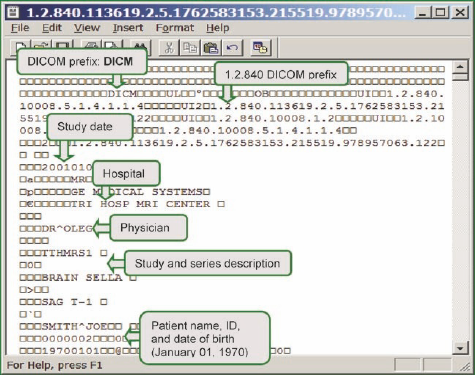
\includegraphics[scale = 0.7]{Content/Pictures/DICOMEditor.png}
	\caption{DICOM Datei in WordPad aus der Patienteninformationen, Krankenhaus und behandelnder Arzt direkt ausgelesen werden können \cite{DICOM}.}
	\label{fig:dicom}
\end{figure}
